\chapter{Tangent Vectors}

\section{Motivation}

Consider the following pictures 
\begin{figure}[H]
    \centering
    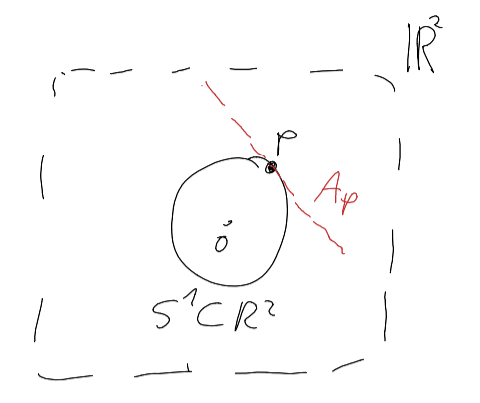
\includegraphics[width=.7\textwidth]{sketch_3_01.png}
    \caption{Sketch 3.01}
\end{figure}
\begin{figure}[H]
    \centering
    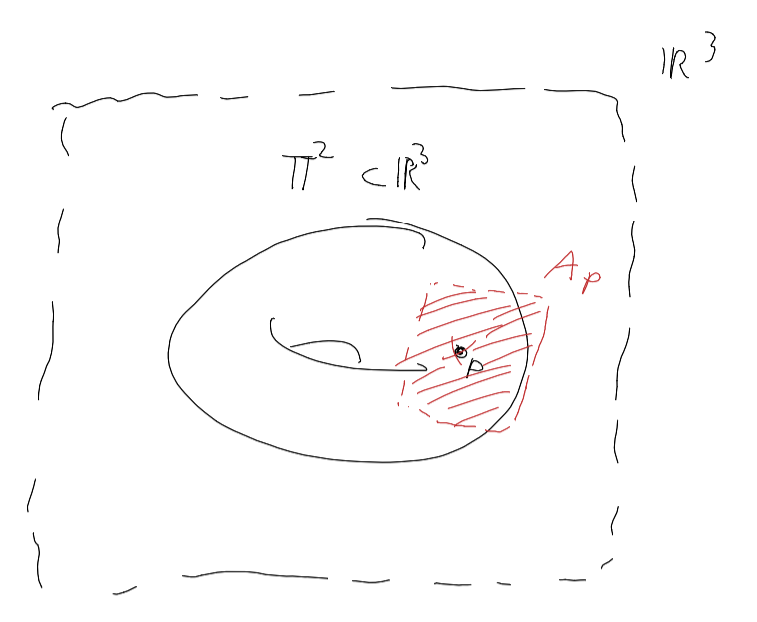
\includegraphics[width=.7\textwidth]{sketch_3_02.png}
    \caption{Sketch 3.02}
\end{figure}
\(A_p\) the affine hyperplane tangent to \(S^1 (\Pi^2)\) at the point \(p\).
Let \(T_p M\coloneqq A_p-p\subset\R^{n+1}\). This is a vector subspace of \(\R^{n+1}\).
It is called the \dhighlight{tangent space of \(M\) at \(p\)}. Consider \[TM=\bigcup_{p\in M} T_pM,\]
called the \dhighlight{tangent bundle}. Observe that there is a map 
\marginnote{Think of \(\pi\) as a map of \(p,T_pM\)}
\[\pi:TM\to M\]
by 
\[x\in T_p M\mapsto p\]
the data \(TM\stackrel{\pi}{\to}\) forms a \dhighlight{vector bundle}.

\dhighlight{Problems with this approach:}

\begin{itemize}
    \item not very intrinsic (depends on \(R^{n+1}\)\dots) 
    \item need to prove that manifolds can always embedded into \(R^N\)
\end{itemize}

This is really the picture / intuition we should have, but we will construct it in a different way.

\section{Two (equivalent) theories of tangent vectors} 

\subsection{Definition via equivalence classes of smooth curves}
\marginnote{I could not quite make out what he called this chapter, so I named it according to 
\cite{taylor_equivalent}}

Let \(M\) be a smooth manifold. Fix \(p\in M\). 
\begin{definition*}
    The \dhighlight{tangent space} of \(M\) at \(p\) denoted by \dhighlight{\(T_pM\)} is 
    the set of equivalence classes of smooth curves \(gamma:[-\epsilon,\epsilon]\to M,\gamma(0)=p\)
    with \(\gamma_1\sim\gamma_2\iff\) for any smooth function \(f\) defined near\footnote{in a neighborhood of} \(p\), we have 
    \((f\circ\gamma_1)'(0)=(f\circ \gamma_2)'(0)\). Here the \(\epsilon>0\) is any positive real number, which depends on \(\gamma\).
\end{definition*} 
\begin{figure}[H]
    \centering
    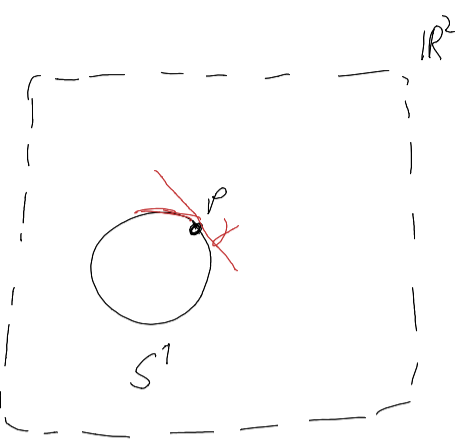
\includegraphics[width=.7\textwidth]{sketch_3_03.png}
    \caption{Sketch 3.03}
\end{figure}

\begin{definition*}
    Given a smooth map \(F:M\to N\), let
    \[dF_p:T_pM\to T_{F(p)}N\]
    be given by \marginnote{This is clearly well defined}
    \[[\gamma]\mapsto [F\circ\gamma].\]
    This map \(dF_p\) is called the \dhighlight{differential of \(F\) at \(p\)}.
\end{definition*}

\begin{remark}
    The map is also called the \dhighlight{tangent map of \(M\) at \(p\)} and the \dhighlight{total derivative}.
    It is also denoted by \[DF_p,TF_p,\nabla F_p,F_p',DF(p),TF(p),\dots\]
\end{remark}

\begin{lemma}[Fundamentality of the differential]\label{lem:3.1}
    Let \(F^1:M_1\to M_2\), \(F^2:M_2\to M_3\) smooth. Then:
    \begin{enumerate}
        \item[(i)]\(dF^2_{F^1(p)}\circ dF_p^1=d(F^2\circ F^1)_p\)
        \item[(ii)] If \(F:M\to M\) is he identity, then \(dF_p=\text{id}\)  
    \end{enumerate}
\end{lemma}

\begin{proof}
    Exercise.
\end{proof}